\documentclass[../document.tex]{subfiles}
\begin{document}
\section{Model}
This section gives an high level overview of the steps in our approach. We will first describe the data gathering,  then the post processing pipeline used to generate the dataset. After, we will introduced the model used to fit the data and then show the results with different test environments.
\subsection{Robot: Krock}
Our task was to apply the approach proposed in \cite{omar@traversability} with a legged robot developed at EPFL named 
\emph{Krock}. Figure \ref{fig:krock} shows the robot in the simulated environment.
\begin{figure}[H]
    \centering
    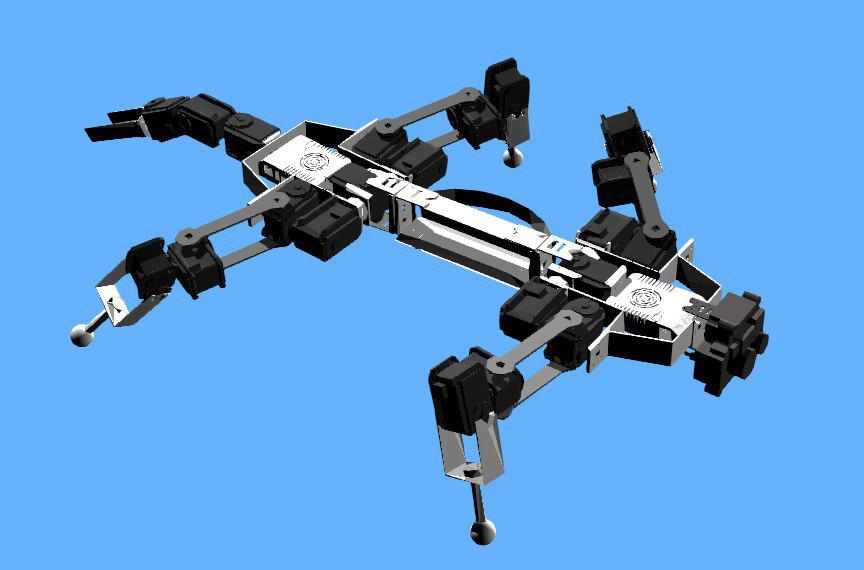
\includegraphics[width=\linewidth]{../img/krock-1.jpg}
    \label{fig:krock}
    \caption{\emph{Krock}}
\end{figure}
Krock has four legs, each one of them is equipped with three motors in order to rotate in each axis. The robot is 
also able to rise itself in three different configurations, gait, using the four motors on the body connected 
to the legs. In addition, there are an other set of two motors in the inner body part to increase krock's moveset. 
The tail is composed by another set of three motors and can be used to perform a wide array of tasks.

The robot is $85cm$ long and it weights around $1.4kg$. Figure \ref{fig:krock-top} shows \emph{Krock} from the top helping the reader 
understanding its composition and the correct ratio between its parts.

\begin{figure}[H]
    \centering
    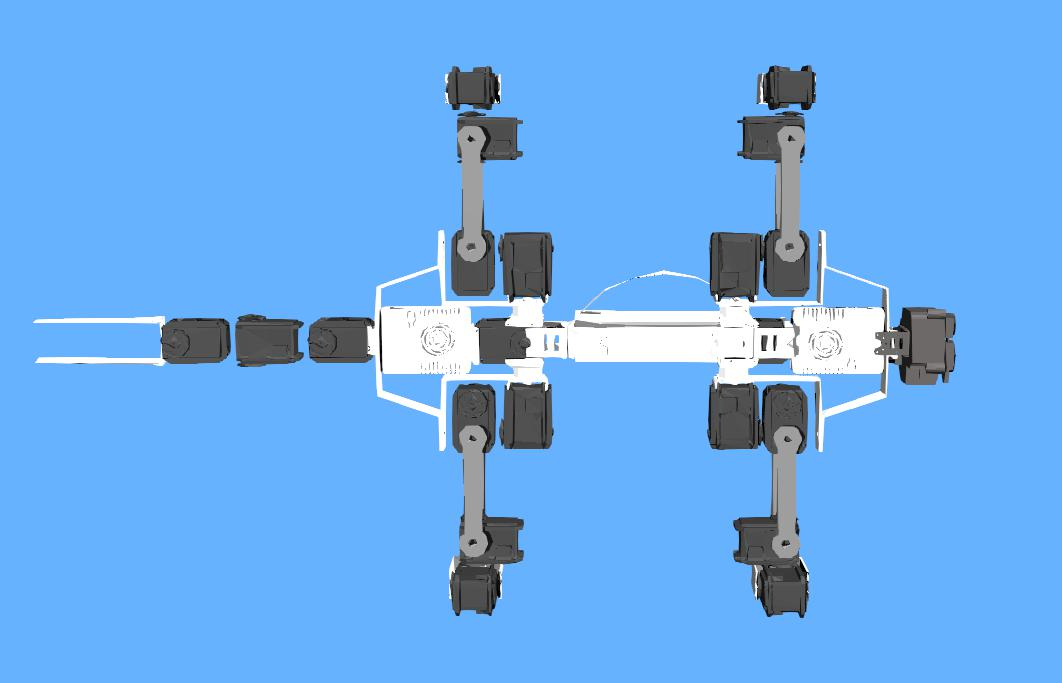
\includegraphics[width=\linewidth]{../img/krock-top.jpg}
    \label{fig:krock-top}
    \caption{Top view of \emph{Krock}}
\end{figure}

\subsection{Simulation}
Our approach relies on simulations to collected the data needed. We used Webots \cite{webots}, a professional 
mobile robot simulator, as backbone of our framework. 

We generate fifteen heighmaps with differens features 
such as walls, bumps and slopes using the same techniques described in \cite{omar@traversability}. Figure \ref{fig:heightmaps}
show some of the maps used in the simulator. 
\begin{figure}[H]
    \todo[inline]{TODO}
\label{fig:heightmaps}
\caption{Some of the heightmaps used in the simulation.}
\end{figure}
\end{document}
